%\documentclass[pdftex,12pt,fullpage,oneside]{amsart}
\documentclass[12pt,fullpage]{article}
\usepackage{array,amsmath,psfrag,amssymb,subfigure,tabularx}
\usepackage{hyperref,multicol}
\usepackage{pa}
\usepackage{booktabs}
%\usepackage{vmargin,boxedminipage}
\usepackage[usenames]{color}
\usepackage{datetime}
\usepackage{dcolumn}
\usepackage{wrapfig}
\usepackage{setspace}
\usepackage{url}
\usepackage[english]{babel}
\usepackage{times}
\usepackage{multirow}
\usepackage[pdftex]{graphicx}
\usepackage{lscape}
\usepackage[top=1in,right=1in,left=1in,bottom=1in]{geometry}
\usepackage{array}
\usepackage{booktabs}
\usepackage{hyperref}

\graphicspath{{/Volumes/"ICEWS Project"/"NSF BMA"/graphics/}} % change to nsf
\newcommand{\note}[1]{\footnote{\doublespacing#1 \vspace{4 mm}}}

\usepackage{natbib}
\bibpunct{(}{)}{;}{a}{}{,}
\bibdata{Flo_Bib}


\title{Improving Predictions Using Ensemble \\ Bayesian Model
  Averaging\thanks{For generously sharing their data and models with
    us, we thank Alan Abramowitz, James Campbell, Robert Erikson, Ray
    Fair, Douglas Hibbs, Michael Lewis-Beck, Andrew D. Martin, Kevin
    Quinn, Stephen Shellman, Charles Tien, \& Christopher Wlezien.
    This project was undertaken in the framework of an initiative
    funded by the Information Processing Technology Office of the
    Defense Advanced Research Projects Agency aimed at producing
    models to provide an Integrated Crisis Early Warning Systems
    (ICEWS) for decision makers in the U.S. defense community. The
    holding grant is to the Lockheed Martin Corporation, Contract
    FA8650-07-C-7749. All the bad ideas and mistakes are our own.  }}
  
\author{
Jacob M. Montgomery\\
	Department of Political Science\\
	Washington University in St. Louis\\
	Campus Box 1063, One Brookings Drive\\
	St. Louis, MO, USA, 63130-4899 
	\and
Florian Hollenbach  \\
	Department of Political Science\\
	Duke University\\
	Perkins Hall 326 Box 90204\\
	Durham, NC, USA, 27707-4330
	\and
Michael D. Ward\\
	Department of Political Science\\
	Duke University\\
	Perkins Hall 326 Box 90204\\
	Durham, NC, USA, 27707-4330\\
	corresponding author: michael.d.ward@duke.edu
} 




\date{\today}


\begin{document}

\maketitle
\thispagestyle{empty}
\clearpage
\pagestyle{myheadings}
\markright{Montgomery, Hollenbach, \& Ward\hfill Ensemble BMA\hfill}

\setcounter{page}{1}
\begin{abstract}
\begin{doublespace}
  We extend ensemble Bayesian model averaging (EBMA) for application
  to binary outcomes and illustrate EBMA's ability to aid scholars in
  the social sciences to make more accurate forecasts of future
  events.  In essence, EBMA makes improves prediction by pooling
  information from multiple forecast models to generate ensemble
  predictions similar to a weighted average of component
  forecasts. The weight assigned to each forecast is calibrated via
  its performance in some training period. The aim is not to choose
  some ``best'' model, but rather to incorporate the insights and
  knowledge implicit in various forecasting efforts via statistical
  postprocessing.  After presenting the method, we show that EBMA
  increases the accuracy of out-of-sample forecasts relative to
  component models in three applied examples: predicting the
  occurrence of insurgencies around the Pacific Rim, forecasting vote
  shares in U.S. presidential elections, and predicting the votes of
  U.S. Supreme Court justices.
\end{doublespace}
\end{abstract}

\doublespacing

\section{Introduction}
Testing systematic predictions about future events against observed
outcomes is generally seen as the most stringent validity check of
statistical and theoretical models.  Yet, political scientists rarely
make predictions about the future.  Empirical models are seldom
applied to out-of-sample data and are even more rarely used to make
predictions about future outcomes. Instead, researchers typically
focus on developing and validating theories that explain past events.

In part, this lack of emphasis on forecasting results from the fact
that it is so difficult to make accurate predictions about complex
social phenomena. However, research in political science could gain
immensely in its policy relevance if predictions were more common and
more accurate.  Improved forecasting of important political events
would make research more germane to policymakers and the general
public who may be less interested in explaining the past than
anticipating and altering the future.  From a scientific standpoint,
greater attention to forecasting would facilitate stringent validation
of theoretical and statistical models since truly causal models should
perform better in out-of-sample forecasting.

In this article, we extend a promising statistical method -- ensemble
Bayesian model averaging (EBMA) -- and introduce software that will
aid researchers across disciplines to make more accurate forecasts.
In essence, EBMA makes more accurate predictions possible by pooling
information from multiple forecast models to generate ensemble
predictions similar to a weighted average of component forecasts. The
weight assigned each forecast is calibrated via its performance in
some training period.  These component models can be diverse.  They
need not share covariates, functional forms, or error
structures. Indeed, the components may not even be statistical models,
but may be predictions generated by agent-based models, stochastic
simulations, or subject-matter experts.

The rest of this article will proceed as follows. We briefly review
existing political science research aimed at forecasting and then
present the mathematical details of the EBMA method. We then
illustrate the benefits of EBMA by applying it to predict insurgency
events on the Pacific Rim, U.S. presidential elections, and voting on
the U.S. Supreme Court.

\section{Dynamic forecasting in political science}
Although forecasting is a rare exercise in political science, there
are an increasing number of exceptions.  In most cases, ``forecasts''
are conceptualized as an exercise in which the predicted values of a
dependent variable are calculated based on a specific statistical
model and then compared with observed values
\citep[e.g.,][]{Hildebrand:etal:1976}. In many instances, this reduces
to an analysis of residuals.  In others, the focus is on randomly
selecting subsets of the data to be excluded during model development
for cross-validation.  However, there is also a more limited tradition
of making true forecasts about events that have not yet occurred.

An early proponent of using statistical models to make predictions in
the realm of international relations (IR) was Stephen Andriole
\citep{Andriole:Young:1977}. In 1978, a volume edited by Nazli Choucri
and Thomas Robinson \nocite{Choucri:Robinson:1978} provided an
overview of the then current work in forecasting in IR.  Much of this
work was done in the context of policy-oriented research for the
U.S. government during the Vietnam War.  Subsequently, there were a
variety of efforts to create or evaluate forecasts of international
conflict including \citet{Freeman:Job:1979},
\citet{Singer:Wallace:1979}, and \citet{Vincent:1980}.  In addition, a
few efforts began to generate forecasts of domestic conflict
\citep[e.g.,][]{Gurr:Lichbach:1986}.  Recent years, however, have
witnessed increasing interest in prediction across a wide array of
contexts in IR.\note{An incomplete list of recent work would include
  \citet{Krause:1997}, \citet{Davies:Gurr:1998},
  \citet{Pevehouse:Goldstein:1999}, \citet{Schrodt:Gerner:2000},
  \citet{King:Zeng:2001}, \citet{OBrien:2002}, \citet{BDM:2002},
  \citet{Fearon:Laitin:2003}, \citet{Demarchi:etal:2004},
  \citet{Enders:Sandler:2005}, \citet{Leblang:Satyanath:2006},
  \citet{Ward:etal:2007}, \citet{Brandt:etal:2008},
  \citet{Bennett:Stam:2009}, and \citet{Gleditsch:Ward:2010}. A
  summary of classified efforts is reported in \citet{Feder:2002}.  An
  overview of some of the historical efforts along with a description
  of current thinking about forecasting and decision-support is given
  by \citet{OBrien:2010}.}  The 2011 special issue of \emph{Conflict
  Management and Peace Science} on prediction in the field of IR
exemplifies this growing emphasis on forecasting
\citep[c.f.,][]{Schneider_etal_2011, Mesquita_2011,
  Brandt_etal_2011}. \citet{wgb:2010} and \citet{Greenhill:2011}
provide additional discussion of forecasting in IR.

Outside of IR, forecasting in political science has largely taken
place in the context of election research.  In the 1990s, scholars of
U.S. politics began publishing predictions of presidential elections
\citep{Campbell:1990, Campbell:1992}. These efforts were anticipated
by the efforts of several economists, most notably the forecasts
established by Ray C. Fair (\citeyear{Fair:1978}). As we discuss
below, predicting U.S. presidential and congressional elections has
since developed into a regular exercise.  Moreover, researchers have
begun to forecast election outcomes in France
\citep[e.g.,][]{Jerome:1999} and the United Kingdom
\citep[e.g.,][]{Whitely:2005}.\note{\citet{Lewis-Beck:2005} provides a
  more in-depth discussion of election forecasting in a comparative
  context.}

While efforts to predict future outcomes remain uncommon, research
that combines multiple forecasts are nearly non-existant.  To our
knowledge, the only non-IR example is the PollyVote project
\citep[c.f.][]{Graefe:2010}, which combines multiple predictions using
simple averages to forecast U.S. presidential elections.

Yet, combining forecasts, and ensemble methods in particular, have
been shown to substantially reduce prediction error in two important
ways.  First, across subject domains, ensemble predictions are usually
more accurate than any individual component model. Second, they are
significantly less likely to make dramatically incorrect predictions
\citep{Bates:1969, Armstrong:2001, Raftery:2005}.  Combining forecasts
not only reduces reliance on single data sources and methodologies
(which lowers the likelihood of dramatic errors), but also allows for
the incorporation of more information than any one theoretical or
statistical model is likely to include in isolation. 

\section{Ensemble Bayesian model averaging} 

Predictive models remain underutilized, yet an increasing number of
scholars have developed forecasting models for specific research
domains.  As the number of forecasting efforts proliferate, however,
there is a growing benefit from developing methods to pool across
models and methodologies to generate more accurate forecasts.  Very
often, specific predictive models prove to be correct only for certain
subsets of observations.  Moreover, specific models tend to be more
sensitive to unusual events or particular data issues than ensemble
methods.

To aid the newfound emphasis on prediction in political science, we
are advancing recent statistical research aimed at integrating
multiple predictions into a single improved forecast.  In particular,
we are adapting an ensemble method first developed for application to
the most mature prediction models in existence -- weather forecasting
models.  To generate predictive distributions of outcomes (e.g.,
temperature), weather researchers apply ensemble methods to forecasts
generated from multiple models \citep{Raftery:2005}.  Thus,
state-of-the-art ensemble forecasts aggregate multiple runs of (often
multiple) weather prediction models into a single unified forecast.

The particular ensemble method we are extending for application to
political outcomes is ensemble Bayesian model averaging (EBMA). First
proposed by \citet{Raftery:2005}, EBMA pools across various forecasts
while meaningfully incorporating \textit{a priori} uncertainty about
the ``best'' model.  It assumes that no particular model or
forecasting method can fully encapsulate the true data-generating
process.  Rather, various research teams or statistical techniques
will reflect different facets of reality. EBMA collects \textit{all}
of the insights from multiple forecasting efforts in a coherent
manner.  The aim is not to choose some ``best'' model, but rather to
incorporate the insights and knowledge implicit in various forecasting
efforts via statistical post-processing.  In recent years, variants of
the EBMA method have been applied to subjects as diverse as inflation
\citep{Wright:2009, Koop:2010, Gneiting:2010}, stock prices
\citep{Billio:2011}, economic growth and policymaking
\citep{Brock:2007, Billio:2010}, exchange rates \citep{Wright:2008},
industrial production \citep{Feldkircher:2010}, ice formation
\citep{Berrocal:2010}, visibility \citep{Chmielecki:2010}, water
catchment streamflow \citep{Viney:2009}, climatology \citep{Min:2006,
  Min:2007, Smith:2009}, and hydrology \citep{Zhang:2009}.  Indeed,
research is underway to extend the method to handle missing data
\citep{Fraley:2010, Mccandless:2011} as well as calibrate model
weights on non-likelihood criteria \citep[e.g.,][]{Vrugt:2006}.

EBMA itself is an extension of the Bayesian model averaging (BMA)
methodology \citep[c.f.,][]{Madigan:1994, Draper:1995, Raftery:1995,
  Hoeting:1999, Clyde:2003, Raftery:2003, Clyde:2004} that has
received considerable attention in the field of statistics. BMA was
first introduced to political science by \citet{Bartels:1997} and has
been applied in a number of contexts \citep[e.g.,][]{Bartels:2001,
  Gill:2004, Imai:2004, Geer:2006b}. \citet{Montgomery:2010c} provide
a more in-depth discussion of BMA and its applications in political
science.



\subsection{Mathematical foundation}

Assume we have some quantity of interest in the future to forecast,
$\mathbf{y}^*$, based on previously collected training data
$\mathbf{y}^T$ that is fit to $K$ statistical models, $M_1, M_2,
\ldots, M_K$. Each model, $M_k$, is assumed to come from the prior
probability distribution $M_k\sim \pi(M_k)$, and the probability
distribution function (PDF) for the training data is
$p(\mathbf{y}^T|M_k)$. The outcome of interest is distributed
$p(\mathbf{y}^*|M_k$).  Applying Bayes Rule, we get that
\begin{equation} \small
p(M_k|\mathbf{y}^T) = \frac{p(\mathbf{y}^T|M_k)\pi(M_k)}{\underset{k=1}{\overset{K}{\sum}}p(\mathbf{y}^T|M_k)\pi(M_k)}.
\end{equation}
\noindent and the marginal predictive PDF for $y^*$ is
\begin{equation}
\label{BMA-pdf}
\small
p(\mathbf{y}^*) = \underset{k=1}{\overset{K}{\sum}} p(\mathbf{y}^*|M_k)p(M_k|\mathbf{y}^T).
\end{equation}
The BMA PDF (\ref{BMA-pdf}) can be viewed as the weighted average of
the component PDFs where the weights are determined by each model's
performance within the training data.  Likewise, we can simply make a
deterministic estimate using the weighted predictions of the
components, denoted
\begin{equation} \small
E(\mathbf{y}^*) = \underset{k=1}{\overset{K}{\sum}} E(\mathbf{y}^*|M_k)p(M_k|\mathbf{y}^T).
\end{equation}

\subsection{EBMA for dynamic settings}

We now turn to applying this basic BMA technology to prediction in a
dynamic setting.  In generating predictions of important events (e.g.,
domestic crises or international disputes), the task is to first build
a statistical model for some set of observations $S$ in time periods
$T$, which we refer to as the training
period.\note{\citet{Sloughter:2007} make predictions for only one
  future time period, and use only a subset of past time-periods (they
  recommend 30) in their training data. Thus, predictions are made
  sequentially with the entire EBMA procedure being re-calculated for
  each future event as observations are moved from the out-of-sample
  period $T^*$ into the training set $T$. Another alternative is to
  simply divide \textit{all} the data into discrete training and test
  periods for the entire procedure.  We use both approaches in our
  examples below.}  Using the same statistical model (or general
technique in the case of subject-expert predictions), we then generate
forecasts, $\mathbf{f}_k$, for observations $S$ in future time periods
$T^*$.

Let us assume, for example, that we have $K$ models forecasting
insurgencies in a set of countries $S$. Each component forecast,
$\mathbf{f}_k$, is associated with a component PDF,
$g_k(\mathbf{y}|\mathbf{f}_k)$, which may be the original predictive
PDF from the forecast model or a bias-corrected forecast.  These
components are the conditional PDFs of outcome $\mathbf{y}$ given the
$k$th forecast, $\mathbf{f}_k$ assuming that $P(M_k | \mathbf{y})
\equiv w_k=1$, or that the posterior odds of model $k$ is unity.

% This
% assumes that $P(M_k | \mathbf{y}) \equiv w_k=1$, or the posterior odds
% of model $k$ is unity.

%  being the ``best''
% forecast in the ensemble. For example, the posterior PDF of an outcome
% $y_{st}$ for some country $s \in S$ in period $t \in T$ given the
% forecast $f_{kst}$ from model $k$ is $g_k(y_{st}|f_{kst})$. 

The EBMA PDF is then a finite mixture of the $K$ component forecasts,
denoted
\begin{equation}
\small
\label{BMA-eq}
p(\mathbf{y}|\mathbf{f}_1, \ldots, \mathbf{f}_K)=\overset{K}{\underset{k=1}{\sum}} w_k
g_k(\mathbf{y}|\mathbf{f}_k),
\end{equation}
\noindent where the weight, $w_k$, is based on forecast $k$'s relative
predictive performance in the training period $T$. The $w_k$'s $\in
[0,1]$ are probabilities and $\sum_{k=1}^Kw_k=1$.  The specific PDF of
for an out-of-sample event, $y_{st^*}$, is therefore
\begin{equation}
\label{BMA-eq2}
\small
p(y_{st^*}|f_{1st^*}, \ldots,
f_{Kst^*})=\overset{K}{\underset{k=1}{\sum}} w_k
g_k(y_{st^*}|f_{kst^*}).
\end{equation}

\subsection{EBMA for normally distributed outcomes}

When forecasting outcomes that are distributed according to the normal
distribution, \citet{Raftery:2005} propose approximating the
conditional PDF as a normal distribution centered at a linear
transformation of the individual forecast, $g_k(\mathbf{y}|\mathbf{f}_k) = N(a_{k0} + a_{k1}\mathbf{f}_k,
\sigma^2)$.  Using \eqref{BMA-eq} above, the EBMA PDF is then
\begin{equation} \small
p(\mathbf{y}|\mathbf{f}_1, \ldots, \mathbf{f}_K) = \overset{K}{\underset{k=1}{\sum}} w_k N(a_{k0} +
a_{k1}\mathbf{f}_k, \sigma^2).
\end{equation}

\subsection{The dichotomous outcome model}

Past work on EBMA does not apply directly to the prediction of many
political events because the assumed PDFs are normal, Poisson, or
gamma. In many settings (e.g., international conflicts), the data are
not sufficiently fine-grained to justify these distributional
assumptions.  Usually, the outcomes of interest are dichotomous
indicators for whether an event (e.g., civil war) has occurred in a
given time period and country. Thus, none of the distributional
assumptions used in past work are appropriate in this context.
Fortunately, it is a straightforward extension of
\citet{Sloughter:2007} and \citet{Sloughter:2010} to deal
appropriately with binary outcomes.\note{The method for dealing with
  binary outcomes is implicit in \citet{Sloughter:2007} and
  \citet{Sloughter:2010}, which assume a discrete-continuous
  distribution for outcomes that include a logistic component.
  However, they do not explicitly and fully develop the model for
  dichotomous outcomes.  A related strain of research on Dynamic Model
  Averaging \citep[c.f.,][]{Raftery:2010, Muhlbaier:2007} has recently
  been extended for direct application to binary outcomes
  \citep[e.g.,][]{Mccormick:2011, Tomas:2011}.}

We follow \citet{Sloughter:2007} and \citet{Hamill:2004} in using
logistic regression after a power transformation of the forecast to
reduce prediction bias. For notational ease, we assume that $\mathbf{f}_k$ is the
forecast after the adjustment for bias reduction.  Therefore, let
$\mathbf{f}'_k \in [0,1]$ be the forecast on the predicted probability scale
 and
\begin{equation}
\small
%\begin{array}{rl}
\mathbf{f}_k =  \left[(1+\mbox{logit}(\mathbf{f}'_k))^{1/b} - 1\right]I\left[\mathbf{f}'_k>\frac{1}{2}\right]  - \left[(1+\mbox{logit}(|\mathbf{f}'_k|))^{1/b} -  1\right]I\left[\mathbf{f}'_k<\frac{1}{2}\right],
%\end{array}
 \end{equation}
 \noindent where $I[.]$ is the general indicator function.
 \citet{Hamill:2004} recommend setting $b=4$, while
 \citet{Sloughter:2007} use $b=3$.  We found that $b=4$ works best in
 the examples below, but other analysts may try alternative
 specifications. This transformation dampens the effect of
   extreme observations and reduces over-fitting.

The logistic model for the outcome variables is % \footnote{Likewise, $\mbox{logit } P(\mathbf{y}=0|\mathbf{f}_k) \equiv
 % \mbox{log}\frac{P(\mathbf{y}=0|\mathbf{f}_k)}{P(\mathbf{y}=1|\mathbf{f}_k)}$.}
\begin{equation} \small
\label{one}
\mbox{logit } P(\mathbf{y}=1|\mathbf{f}_k) \equiv \mbox{log}\frac{P(\mathbf{y}=1|\mathbf{f}_k)}{P(\mathbf{y}=0|\mathbf{f}_k)} = a_{k0}+a_{k1}\mathbf{f}_k .
\end{equation}
\noindent The conditional PDF of some within-sample event, given the
forecast $f_{kst}$ and the assumption that $k$ is the true model, can
be written
\begin{equation} 
\label{component-eq}
\small
g_k(y_{st}|f_{kst}) = P(y_{st}=1|f_{kst})I[y_{st}=1]  + P(y_{st}=0|f_{kst})I[y_{st}=0].
\end{equation}
Applying this to \eqref{BMA-eq}, the PDF of the final EBMA model for
$y_{st}$ is
\begin{equation}
\label{pdf}
\small
\begin{array}{rl}
p(y_{st}|f_{1st}, f_{2st}, \ldots, f_{Kst}) = &
\overset{K}{\underset{k=1}{\sum}} w_k [
P(y_{st}=1|f_{kst})I[y_{st}=1] \\
& + P(y_{st}=0|f_{kst})I[y_{st}=0]].\end{array}
\end{equation}

\subsection{Parameter estimation by maximum likelihood and EM
algorithm}

Parameter estimation is conducted using only the data from the
training period $T$.  The parameters $a_{0k}$ and $a_{1k}$ are
specific to each individual component model.  For model $k$, these
parameters can be estimated as traditional linear models where
$\mathbf{y}$ is the dependent variable and the covariate list includes
only $\mathbf{f}_k$ and a constant term.

The difficulty is in estimating the weighting parameters,
$w_k~\forall~ k \in [1, 2, \dots, K]$. For the moment, we have
followed \citet{Raftery:2005} and \citet{Sloughter:2007} in using
maximum likelihood methods. In future work we plan to implement a
fully Bayesian analysis by placing priors on all parameters and using
Markov chain Monte Carlo techniques to estimate model weights
\citep[c.f.][]{Vrugt:2008}.

With standard independence assumptions, the log-likelihood for the
model weights is
\begin{equation}
\small
  \ell (w_1, \ldots, w_K | a_{01},  \ldots, a_{0K}; a_{11},
  \ldots, a_{1K})= \underset{s,t}{\sum}\mbox{log }p(y_{st} |
  f_{1st}, \ldots, f_{Kst}).
\end{equation}
\noindent where the summation is over values of $s$ and $t$ that index
all observations in the training time period, and $p(y_{st}|f_{1st},
\ldots, f_{Kst}) $ is given by \eqref{pdf}. The log-likelihood
function cannot be maximized analytically, but \citet{Raftery:2005}
and \citet{Sloughter:2007} suggest using the expectation-maximization
(EM) algorithm.  We introduce the unobserved quantities $z_{kst}$,
which represent the posterior probability for model $k$ for
observation $y_{st}$.  The E step involves calculating estimates for
these unobserved quantities using the formula
\begin{equation}
\small
\hat{z}^{(j+1)}_{kst} = \frac{\hat{w}^{(j)}_k
p^{(j)}(y_{st}|f_{kst})}{\overset{K}{\underset{k=1}{\sum}}\hat{w}^{(j)}_kp^{(j)}(y_{st}|f_{kst})},
\end{equation}
\noindent where the superscript $j$ refers to the $j$th iteration of
the EM algorithm.

It follows that $w_k^{(j)}$ is the estimate of $w_k$ in the $j$th
iteration and $p^{(j)}(.)$ is shown in \eqref{pdf}.  Assuming these
estimates of $z_{kst}$ are correct, it is then straightforward to
derive the maximizing value for the model weights. Thus, the M step
estimates these as
$\hat{w}^{(j+1)}_k=\frac{1}{n}\underset{s,t}{\sum}\hat{z}^{(j+1)}_{kst}$,
where $n$ represents the number of observations in the training
dataset.\note{In the case of normally distributed data,
  $\hat{\sigma}^{2(j+1)}=\frac{1}{n}\underset{s,t}{\sum}\overset{K}{\underset{k=1}{\sum}}\hat{z}^{(j+1)}_{kst}(y_{st}-f_{kst})^2$.}
The E and M steps are iterated until the improvement in the
log-likelihood is no larger than some pre-defined
tolerance.\note{Although the log-likelihood will increase after each
  iteration of the algorithm, convergence is only guaranteed to a
  local maximum of the likelihood function.  Convergence to the global
  maximum is not assured, and the model may be sensitive to initial
  conditions. In future research, we will explore these convergence
  issues more fully with special attention paid to comparison with
  fully Bayesian implementations. In the examples below, we begin with
  the assumption that all models are equally likely, $w_k =
  \frac{1}{K} ~ \forall ~ k \in [1, \ldots, K]$.}



\subsection{Ensemble prediction}

With these parameter estimates, it is now possible to generate
ensemble forecasts. If our forecasts, $\mathbf{f}_k$, are generated
from a statistical model, we now generate a new prediction,
$f_{kst^\ast}$, from the previously fitted models. For convenience,
let $\hat{\mathbf{a}}_k \equiv (\hat{a}_{k0}, \hat{a}_{k1})$. For some
dichotomous observation in country $s\in S$ in the out-of-sample
period $t^\ast\in T^\ast$, we can see that
\begin{equation}
\label{nothing}
{\small
P(y_{st^*} = 1 | f_{1st^\ast}, \ldots, f_{Kst^\ast} ;  \hat{\mathbf{a}}_1,
 \ldots, \hat{\mathbf{a}}_K ; \hat{w}_1, \ldots, \hat{w}_K) =
 \overset{K}{\underset{k=1}{\sum}} \hat{w}_k
 \mbox{logit}^{-1}\left(\hat{a}_{k0} +  \hat{a}_{k1}f_{kst^\ast}\right).}
\end{equation}


\section{Empirical applications}

\subsection{Application to insurgency forecasting}

Our first example applies the EBMA method to data
collected for the Integrated Crisis Early Warning Systems (ICEWS)
project sponsored by the Defense Advanced Research Projects Agency
(DARPA).  The task of the ICEWS project is train models on data
(focusing on five outcomes of interest) for 29 countries for every month from 1997
through the present and to then make accurate predictions about
expected crisis events over the subsequent three months.\note{The
  twenty-nine countries are Australia, Bangladesh, Bhutan, Cambodia,
  China, Comoros, Fiji, India, Indonesia, Japan, Laos, Madagascar,
  Malaysia, Mauritius, Mongolia, Myanmar, Nepal, New Zealand, North
  Korea, Papua New Guinea, Philippines, Russia, Singapore, Solomon
  Islands, South Korea, Sri Lanka, Taiwan, Thailand, and Vietnam. This
  set is not a random sample, but rather constitutes the countries of
  population greater than $500,000$ that are in the area of
  responsibility of the US Pacific Command.}  For purposes of
demonstration, we focus on only one of these outcomes -- violent
insurgency.

The bulk of the data for the ICEWS project is gleaned from natural
language processing of a continuously updated harvest of news stories
(primarily taken from Lexus/Nexus and Factiva archives). These are
digested with a version of the TABARI processor for events developed
by Philip Schrodt and colleagues in the context of the Event Data
Project (see \url{http://eventdata.psu.edu/} for more details).  These
data are augmented with a variety of covariates including:
country-level attributes (coded on a monthly or yearly basis) from the
Polity and World Bank datasets, information about election cycles (if
any), events in neighboring countries, and the length of shared
borders with neighboring countries.

\subsubsection{Component models:}

In the remainder of this subsection, we apply EBMA to make predictions
for the occurrence of insurgency in these 29 countries.  We estimate
three exemplar statistical models using data for the in-sample period
ranging from January 1999 to December 2008 and fit an EBMA model.  We
then make out-of-sample forecasts for the period from January 2009 to
December 2010 for the component and EBMA models.  To provide variation
in the complexity (as well as accuracy) of the components, we included
the following models.

\begin{list}{\labelitemi}{\leftmargin=1em}
\item \textbf{SAE}: This is one model developed as part of the ICEWS
  project and was designed by Strategic Analysis Enterprises. It is
  specified as a simple generalized linear logistic model including 27 different
  independent variables.\note{See
    \url{strategicanalysisenterprises.com} for more details.  All data
    and models will be included in a replication dataset at the time
    of publication.}  All of the variables are taken from the ICEWS
  event-stream data.
\item \textbf{GLM}: For the purposes of demonstrating the properties
  of the EBMA method, we estimated a crude logistic model that
  includes only \textit{population size} and \textit{GDP growth} (both
  lagged three months).
\item \textbf{LMER}: This is a generalized linear mixed effects model
  using a logistic link function and including random country-level
  intercepts. In addition to the variables from the GLM model, the
  list of covariates includes: the \textit{executive constraint} and
  \textit{competitiveness of participation} variables from the Polity
  IV dataset \citep{PolityIV}, \textit{proximity to
    election},\note{This is calculated as the number of days to the
    next or from the last election, whichever is closer.} and a
  \textit{spatial lag} that reflects recent occurrences of
  insurgencies in the countries' geographic
  neighbors.\note{Geographical proximity is measured in terms of the
    length of the shared border between the two countries.}
\end{list}

\subsubsection{Results:}

Table \ref{InSam1} shows the EBMA model parameters as well as fit
statistics associated with the individual component models and the
EBMA predictions for the in-sample time period. The first column shows
the weights that the EBMA model assigned to each component. As can be
seen, the GLM model is effectively excluded, while the SAE model
carries the greatest weight followed by the LMER model.  The constant
term associated with each component corresponds to the term $a_{k0}$
in (\ref{one}), while the predictor corresponds to $a_{k1}$.
The other columns in Table \ref{InSam1} are fit statistics.  AUC is
the area under the Receiver-Operating Characteristic (ROC) curve. The
advantage of using ROC curves is that it evaluates forecasts in a way
that is less dependent on an arbitrary cutoff point.  A value of 1
would mean that all observations were predicted correctly at all
possible cutoff points \citep{King:Zeng:2001}.

\begin{table}[h!]
\small
% latex table generated in R 2.12.0 by xtable 1.5-6 package
% Thu May 12 10:47:15 2011
\begin{center}
  \caption{\footnotesize In-sample results.  The table shows estimated
    model weights, parameters, and fit statistics for the EBMA
    deterministic forecast and all component forecasts of insurgency
    in 29 countries of the Pacific Rim.  EBMA equals or outperforms
    any single model on all measures.}\label{InSam1}
\begin{tabular}{lrrrrrrrrr}
  \toprule
 & Weight & Constant & Predictor & AUC & PRE & Brier & \% Correct \\ 
  \midrule
  SAE & 0.57 & 0.04 & 7.46 & 0.96 & 0.48 & 0.04 & 94.11\\ 
  LMER & 0.43 & 6.08 & 28.25 & 0.96 & 0.01 & 0.07 & 88.79\\ 
  GLM & 0.00 & 0.57 & 8.16 & 0.65 & 0.00 & 0.10 & 88.65\\ 
  EBMA &  &  &  & 0.97 & 0.55 & 0.04 & 94.94\\ 
   \bottomrule
n=3,480\\
\end{tabular}
\end{center}
\end{table}


We compare the models using three additional metrics.  The
proportional reduction in error (PRE) is the percentage increase of
correctly predicted observations relative to some pre-defined base
model. In this case, the base model is predicting ``no insurgencies''
for all observations.  Insurgencies are relatively rare events.  Thus,
predicting a zero for all observations leads to an 89\% correct
prediction rate. The Brier score is the average squared deviation of
the predicted probability from the true event (0 or 1).  Thus, a lower
score corresponds to higher forecast accuracy \citep{Brier:1950}.
Finally, we calculate the percentage of observations that each model
would predict correctly using a 0.5 threshold on the predicted
probability scale.
\begin{figure}
%\begin{wrapfigure}{L}{.5\textwidth}
  \caption{\footnotesize Separation plots for in-sample predictions of
    the ICEWS data (n=3,480).  For each model, observations are shown
    from left to right in order of increasing predicted probability of
    insurgency (shown as the black line).  Observations where
    insurgency actually occurred are shown in red. EBMA outperforms
    all component models in assigning high predicted probabilities to
    \textit{more} observed insurgencies and to \textit{fewer}
    non-insurgencies.}
\label{InSam1sep}
\begin{center}
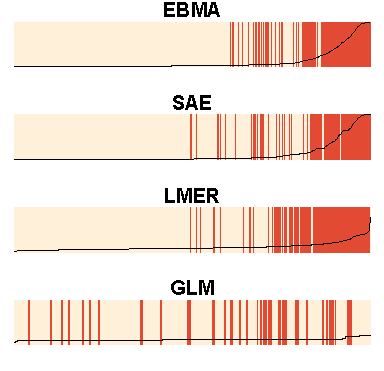
\includegraphics[]{Insamplenew.pdf}
\end{center}
%\end{wrapfigure}
\end{figure}

There are two aspects of Table \ref{InSam1} that are important to
note.  First, the EBMA model does at least as well (and usually
better) than all of the component models on each our model fit
statistics.  The EBMA model has the highest AUC, PRE, and \% correct.
In addition, it is tied for the lowest Brier score with the SAE model.
Second, in this example the EBMA procedure assigns probability weights
to each model according to their in-sample performance.  The largest
model weight (0.57) is assigned to the SAE model, which appears to be
the best (or tied for the best) component as measured by all of our
fit statistics. Meanwhile, the smallest weight (0.00) is assigned to
the rudimentary GLM model.

Figure \ref{InSam1sep} shows separation plots for the EBMA model and
the individual components \citep{Greenhill:2011}. In each plot, the
observations are ordered from left to right by increasing predicted
probabilities of insurgency (as predicted by the particular
model). The black line corresponds to the predicted probability
produced by the relevant model for each observation and actual
occurrences of insurgencies are colored red.  Figure \ref{InSam1sep}
shows visually that the GLM model performs very poorly, whereas of the
SAE model is the best component.  More importantly, the overall best
performance is associated with the EBMA forecast. The separation plots
show that the EBMA model produces few false positives and even fewer
false negatives than any of the component models.

\begin{table}[h!]
\small
\begin{center}
  \caption{\footnotesize Out-of-sample results.  The table shows fit
    statistics for the EBMA deterministic forecast and all component
    model forecasts of insurgency in 29 countries of the Pacific Rim.
    EBMA equals or outperforms any single model on most
    measures.}\label{OutSam1}
\begin{tabular}{lrrrrr}
  \toprule
 & AUC & PRE & Brier & \% Correct   \\ 
  \midrule
  SAE &  0.96 & 0.04 & 0.06 & 89.80   \\ 
  LMER & 0.97 & 0.00 & 0.07 & 89.37  \\ 
  GLM & 0.84 & 0.00 & 0.09 & 89.37  \\ 
  EBMA & 0.96 & 0.18 & 0.05 & 91.24 \\ 
   \bottomrule
n=696 \\
\end{tabular}
\end{center}
\end{table}

The more interesting evaluation of the EBMA method is its
out-of-sample predictive power. Table \ref{OutSam1} shows fit
statistics for the individual components as well as the EBMA forecasts
for observations in the 24 months following the training period.
While the EBMA model has a marginally smaller area under the ROC curve
than the LMER models, it outperforms all component models on the other
metrics. In particular, the EBMA model has the highest PRE at 0.18.
Since it is possible to predict 89.22\% of these observations
correctly by forecasting no insurgency, an 18\% reduction of error
relative to the baseline model is quite substantial.

Figure \ref{OutSam1sep} shows the separation plots for the components
as well as the EBMA forecasts for the out-of-sample data.  The EBMA
model again performs better than any of the individual components with
very high predicted probabilities for the majority of actual events.
Taking both the fit statistics and the visual evidence together, we
can conclude that the EBMA model leads to a substantial improvement in
out-of-sample forecasts relative to its components.  This is true even
in datasets with rare events and even when the individual components
are already performing well.


\begin{figure}
%\begin{wrapfigure}{L}{0.5\textwidth}
  \caption{\footnotesize Separation plots for out-of-sample
    predictions of the ICEWS data (n=696).  For each model,
    observations are shown from left to right in order of increasing
    predicted probability (shown as the black line).  Observations
    where insurgency actually occurred are shown in red.  EBMA
    outperforms all component models in assigning high predicted
    probabilities to \textit{more} observed insurgencies and to
    \textit{fewer} non-insurgencies.}
\label{OutSam1sep}
\begin{center}
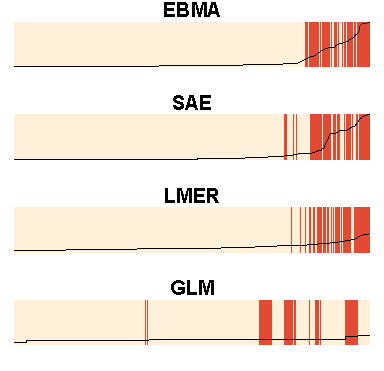
\includegraphics[]{OutSampleNew.pdf}
\end{center}
%\end{wrapfigure}
\end{figure}


\subsection{Application to US presidential election forecasts}
For the past several U.S. election cycles, a number of research teams
have developed forecasting models and published their predictions in
advance of Election Day.  For example, before the 2008 election, a
symposium of forecasts was published in \emph{PS: Political Science
  and Politics} with forecasts of presidential and congressional vote
shares developed by \citet{Campbell:2008}, \citet{Norpoth:2008},
\citet{Lewis-Beck:Tien:2008}, \citet{Abramowitz:2008},
\citet{Erikson:Wlezien:2008}, \citet{Holbrook:2008},
\citet{Lockerbie:2008} and \citet{Cuzan:Bundrick:2008}.  Responses to
the forecast were published in a subsequent issue. Earlier, in 1999,
an entire issue of the \textit{International Journal of Forecasting}
was dedicated to the task of predicting presidential elections
\citep{Brown:1999}.  Predicting presidential elections has also drawn
the attention of economists seeking to understand the relationship
between economic fundamentals and political outcomes.  Two prominent
examples include work by Ray Fair (\citeyear{Fair:2010}) and Douglas
Hibbs (\citeyear{Hibbs:2000}).

\subsubsection{Component models:}

In the rest of this subsection, we replicate several of these models and
demonstrate the usefulness of the EBMA methodology for improving the
prediction of single important events.  We include six of the most widely cited
presidential forecasting models.
\begin{list}{\labelitemi}{\leftmargin=1em}
\item \textbf{Campbell}: Campbell's ``Trial-Heat and Economy Model''
  \citep{Campbell:2008}
\item \textbf{Lewis-Beck/Tien}: Lewis-Beck and Tien's ``Jobs Model Forecast'' \citep{Lewis-Beck:Tien:2008}
\item \textbf{Erikson/Wlezien}: Erikson and Wlezien's ``Leading Economic Indicators
  and Poll'' forecast\note{We replicated Column 2 in Table 2 from \citet{Erikson:Wlezien:2008}.}
\item \textbf{Fair}: Fair's presidential vote-share model\note{The model here replicates Equation 1 in \citet{Fair:2010}.}
\item \textbf{Hibbs}: Hibbs' ``Bread and Peace Model'' \citep{Hibbs:2000}
\item \textbf{Abramowitz}: The ``Time-for-Change Model'' created by
  \citet{Abramowitz:2008}
\end{list}
\noindent With the exception of the Hibbs forecast, the models are
simple linear regressions. The dependent variable is the share of the
two-party vote received by the incumbent-party candidate.\note{The
  data to replicate the models by \citet{Abramowitz:2008},
  \citet{Campbell:2008}, \citet{Erikson:Wlezien:2008}, and
  \citet{Lewis-Beck:Tien:2008} were provided in personal
  correspondence with the respective authors.  The remaining data were
  downloaded from the web sites of Ray C. Fair \nocite{Fair2011} and
  Douglas Hibbs \nocite{Hibbs2011}.}


\subsubsection{Results:}

Rather than selecting a single training period (as in the insurgency
analysis) we generate sequential predictions.  For each year from 1976
to 2008, we use all available prior data to fit the component
models.\note{For example, the Fair model uses data for election
  results beginning in 1916 while the Abramowitz model begins with
  data from the 1952 election. }  We then fit the EBMA model using the
components' in-sample performances for election years beginning with
1952 (the year when all models begin generating predictions).  For
example, to generate predictions for the 1988 election, we used the
in-sample performance of each component for the 1952-1984 period to
estimate model weights.\note{Results in this section were computed
  using modifications of the `ensembleBMA' package
  \citep{Fraley:2010b, Fraley:Forthcoming}.  Because of the paucity of
  data, we did not apply any bias correction to these forecasts.  Thus,
  the predictor and constant, denoted $a_{0k}$ and $a_{1k}$ above, are
  constrained to zero and one respectively.}


% \begin{table}[ht!]
%   \caption{\footnotesize Prediction errors, model weights, and in-sample fit
%     statistics for component and EBMA forecasts of the 2008 and 2004
%     elections.  Models are sequentially fit using all prior elections.
%     The EBMA model does better than all components on in-sample fit
%     statistics.  Although it does not necessarily make the most accurate
%     prediction for any given year, it is less likely to make
%     dramatic forecasting errors.}
% \label{Pres-Year-Res} \small
% \begin{center}
% \begin{tabular}{l rrrrrrrr}	
%   \toprule
%   &\multicolumn{4}{c}{\textit{2008 Election}}  &\multicolumn{4}{c}{\textit{2004 Election}} \\ 
%   &\shortstack{Pred. \\ Error} &	Weights&	RMSE &MAE & \shortstack{Pred.\\  Error} &Weights&	RMSE&	MAE\\
%   \midrule
%   Campbell            &	6.33 &	0.36	 & 1.65&	1.28	&
%   0.53 & 0.40 & 1.71 & 1.33\\
%   Lewis-Beck/Tien &	-2.65 &	0.17	&1.61&	1.33	&	-0.41 &
%   0.00 & 1.67 & 1.42\\
%   Erikson/Wlezien &	-0.14 &	0.17 & 2.81 & 	2.18	&	4.76 &
%   0.00 & 2.67 & 2.06\\
%   Fair                      &	-2.02 &	0.00	&2.22&	1.80	&
%   4.82 & 0.48 & 2.07 & 1.47\\
%   Hibbs                   & -1.39 &	0.25	&1.92&	1.38	&
%   1.54 & 0.12 & 1.95 & 1.38\\
%   Abramowitz        &	-2.37 &	0.06	& 1.53 &	1.26	&
%   2.20 &
%   0.00 & 1.50  & 1.18\\
%   EBMA                    &	-0.53&	        &1.30&	1.01	&
%   2.08	&       & 1.29 & 1.01\\
%   \bottomrule
% \end{tabular}
% \end{center}
% \end{table}

\begin{table}[ht!]
  \caption{\footnotesize Prediction errors, model weights, and in-sample fit
    statistics for component and EBMA forecasts of the 2004 and 2008
    elections.  Models are sequentially fit using all prior elections.
    The EBMA model does better than all components on in-sample fit
    statistics.  Although it does not necessarily make the most accurate
    prediction for any given year, it is less likely to make
    dramatic forecasting errors.}
\label{Pres-Year-Res} \small
\begin{center}
\begin{tabular}{l rrrrrrrr}	
  \toprule
   &\multicolumn{4}{c}{\textit{2004 Election}} &\multicolumn{4}{c}{\textit{2008 Election}} \\ 
 &	Weights&	RMSE &MAE &\shortstack{Pred. \\ Error}
 &Weights&	RMSE&	MAE &  \shortstack{Pred.\\  Error}\\
\midrule
 Campbell               &0.40&1.71&1.33 &0.53&0.36&1.65&1.28&6.33\\
  Lewis-Beck/Tien 	&0.00&1.67&1.42&$-$0.41&	0.17&1.61&1.33&$-$2.65\\
  Erikson/Wlezien 	&0.00&2.67&2.06&4.76&0.17&2.81&2.18&$-$0.14\\
  Fair                      	&0.48&2.07&1.47&4.82&0.00&2.22&1.80&$-$2.02 \\
  Hibbs                   	&0.12&1.95&1.38&1.54&0.25&1.92&1.38&$-$1.39\\
  Abramowitz        	&0.00&1.50&1.18&2.20&0.06&1.53&1.26&$-$2.37\\
  EBMA                    	&	       	&1.29&1.01&2.08&
  &1.30&1.01&$-$0.53\\
\bottomrule
\end{tabular}
 \end{center}
 \end{table}



Table \ref{Pres-Year-Res} provides exemplar results for the 2004 and 2008
elections.  Table \ref{Pres-Year-Res} shows the
weights assigned to each model as well as the in-sample root mean
squared error (RMSE) and mean absolute error (MAE) for the components
and the EBMA forecasts.   The table also shows the out-of-sample prediction
errors, calculated as $y_{predicted}-y_{observed}$, for each component
model and the EBMA forecast.

% It is helpful here to visualize the EBMA predictive PDF and its
% components for these two exemplar years.  A representation of the EBMA
% model for these years is shown in Figure \ref{PresPlots}.  The thin
% colored lines represent the predictive PDFs of the component
% forecasts.  Their relative weight in the final EBMA predictive PDF is
% represented by their relative height.  The sum of these weighted
% components is therefore the solid black lines, which is the final EBMA
% predictive PDF.  In addition, the EBMA deterministic forecast (the
% ``O'') and its 95\% predictive interval (the dashed line) are plotted
% against the true observed electoral outcome (the ``X'') for these two
% exemplar years.


%  \begin{figure}[ht!]
%    \caption{\footnotesize Weighted predictive PDF's for component
%      models (colored lines) and the full EBMA predictive PDF (thick
%      black line).  The ``O'' shows the deterministic EBMA prediction
%      and the ``X'' shows the actual observed value for the given year.
%      The dashed line is the 95\% credible interval for the EBMA
%      predictive PDF.  The EBMA predictive PDF is the weighted
%      combination of component PDFs.}
%  \label{PresPlots}
%  \begin{center}
%  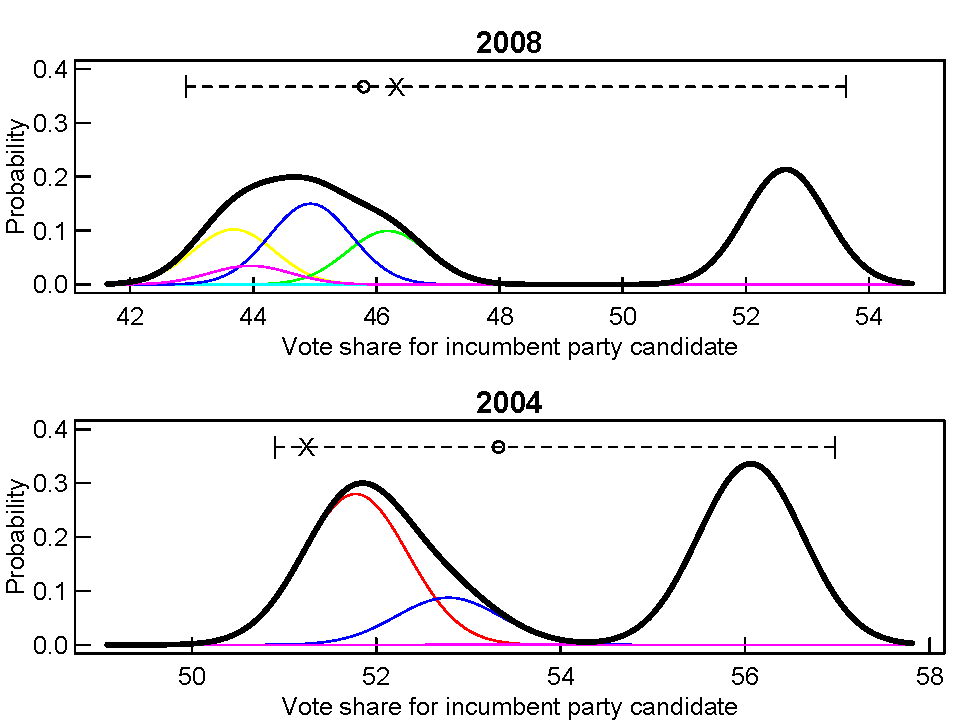
\includegraphics[width=5 in]{PresPlots.PDF}
%  \end{center}
%  \end{figure}


The example results in Table \ref{Pres-Year-Res} illustrate three
important points.  First, the EBMA model again does better than any
individual component on in-sample measures of model fit (i.e., RMSE
and MAE).  Second, these results demonstrate that EBMA is not
guaranteed to generate the most accurate prediction for any single
observation.  Thus, in each year some component models come closer to
predicting the actual outcome.  However, the EBMA forecasts will very
rarely provide egregiously wrong predictions (e.g., the Campbell model
in 2008 and the Fair model in 2004) since it borrows predictions from
multiple components.  Moreover, as we show below, in the aggregate the
EBMA model tends to provide the best forecast over time.

Third, Table \ref{Pres-Year-Res} shows it is clear that there is
not as clean a relationship between in-sample model performance and
model weights as in the insurgency example.  For instance, the weight
for the Abramowitz model in 2008 is 0.06 even though it has the lowest
RMSE and MAE of any component.  The diminished relationship between
in-sample performance and weight is a result of high in-sample
correlations between forecasts.\note{The correlation matrix between
  fitted-values of the model for the
  1952-2008 period is: \\
\begin{tabular}{l  rrrrrr}
  \toprule
 & \textbf{C}& \textbf{L} & \textbf{E}& \textbf{F} & \textbf{H} & \textbf{A} \\ 
  \midrule
\textbf{C}ampbell& 1.00 & & & & & \\ 
 \textbf{L}ewis-Beck/Tien& 0.93 & 1.00 & & & & \\ 
\textbf{E}rikson/Wlezien & 0.85 & 0.86 & 1.00 & & & \\ 
\textbf{F}air & 0.87 & 0.88 & 0.91 & 1.00 & & \\ 
\textbf{H}ibbs& 0.91 & 0.91 & 0.87 & 0.89 & 1.00 & \\ 
\textbf{A}bramowitz & 0.94 & 0.96 & 0.90 & 0.90 & 0.93 & 1.00 \\ 
   \bottomrule
 \end{tabular}.}  For
instance, fitted values for the Abramowitz model are correlated at
0.94 with the Campbell model and at 0.96 with the Lewis-Beck/Tien
model. Thus, conditioned on knowing these forecasts, the Abramowitz
component provides limited additional information.  

With the 2004 and 2008 examples in mind, we now turn to the relative
out-of-sample performance of the EBMA and component forecasts across
the entire 1976-2008 period.  Table \ref{Pres-Res} shows the
out-of-sample RMSE and
MAE statistics as well as the percentage of observations that fall
within the 67\% and 95\% predictive intervals for each.  For our
purposes here, the main result in Table \ref{Pres-Res} is that the
EBMA model again outperforms all components.  The first two columns
show this to be true in terms of predicted error (RMSE and MAE).


\begin{table}[ht!]
  \caption{\footnotesize Fit statistics and observed coverage
    probabilities for sequentially generated out-of-sample predictions of
    presidential elections from 1976-2008.  EBMA outperforms its
    component models on all metrics.}
\label{Pres-Res} \small
\begin{center}
\begin{tabular}{lrrrrr}
\toprule
                        &              &              & \multicolumn{2}{c}{Coverage} \\ 
                    	&	RMSE&	MAE	&67\% &   90\%      \\
\midrule
EBMA	           &	1.72	&	1.47	&	0.67	&	0.89	\\
Campbell	           &	2.74	&	1.99	&	0.67	&	0.78	\\
Lewis-Beck/Tien&	2.27	&	1.82	&	0.89	&	1.00	\\
Erikson/Wlezien&	2.88	&	2.16	&	0.78	&	1.00	\\
Fair	                   &	4.01	&	3.20	&	0.44	&	0.78	\\
Hibbs	           &	2.81	&	2.24	&	0.44&      0.78 \\
Abramowitz	   &	2.27	&	2.05	&	0.33	&     0.78	\\

\bottomrule
\end{tabular}
\end{center}
\end{table}



 \begin{figure}[ht!]
   \caption{\footnotesize The predicted and actual percentage of the
     two-party vote going to the incumbent party in U.S. presidential
     elections from six component models and the EBMA forecast.  For
     each year, the plots show the point predictions (circles), 67\%
     predictive intervals (thick horizontal lines), and 90\%
     predictive intervals (thin horizontal lines).  The vertical
     dashed line is the observed outcome.  The EBMA model is
   better calibrated than its components.  Specifically, the
   models at the bottom of each plot generate relatively wide
   predictive intervals.}
 \label{PresPlots2}
 \begin{center}
 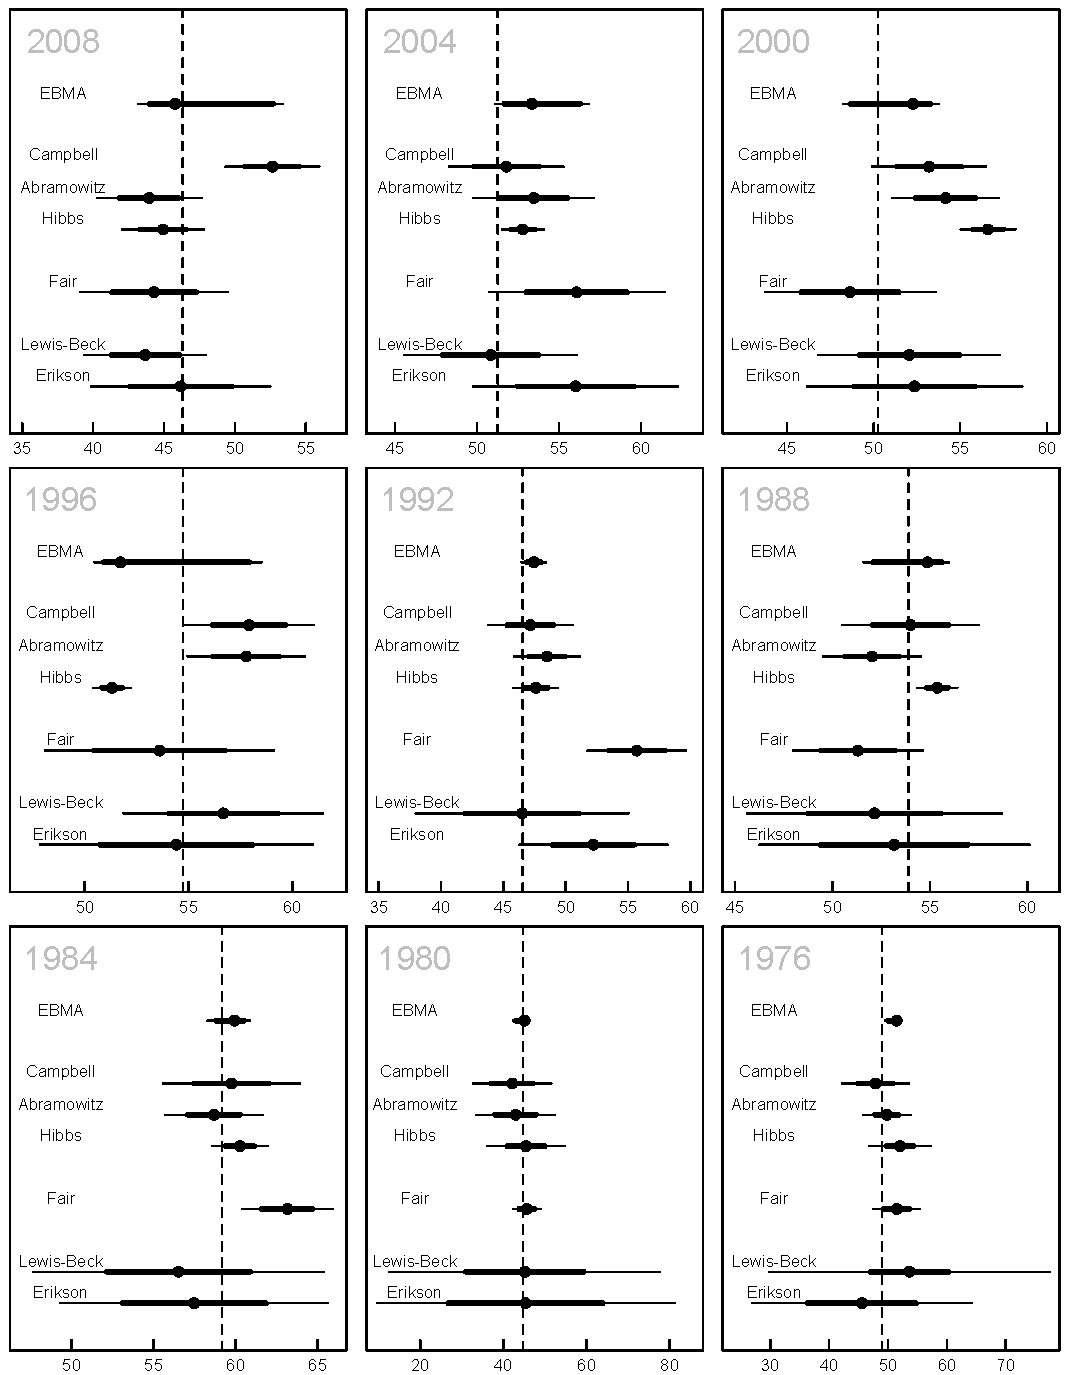
\includegraphics[width=5.6 in]{PresPlot2.PDF}
 \end{center}
 \end{figure}


 In addition, the coverage statistics demonstrate better calibration
 of EBMA forecasts relative to its component models.  For instance,
 the observed outcome falls within the 67\% predictive interval for
 the Abramowitz model only three out of nine times, while it covers the
 observed values eight out of nine times for the Lewis-Beck/Tien
 model.  Meanwhile, the EBMA 90\% an 67\% predictive intervals are
 nearly perfectly calibrated.

 In a well-calibrated forecasting model, out-of-sample outcomes should
 fall within predictive intervals at a rate corresponding to their
 size.  For instance, the goal is for two-thirds of all out-of-sample
 observations to fall within of their respective 67\% predictive
 intervals.  Poorly calibrated models will tend to be produce
 predictive intervals that are either too narrow, generating
 inaccurate predictions, or too large, generating predictions that are
 accurate but too vague to be useful.  The better calibration of the
 EBMA model can be seen visually in Figure \ref{PresPlots2}.  The plot
 shows the point predictions and the 67\% and 90\% predictive
 intervals for each model in each year.  The vertical dashed lines
 show the actual observed outcomes.  Note that two of the most
 accurate forecasts, the Lewis-Beck/Tien and Erikson/Wlezien models,
 make very imprecise predictions.  Thus, although they have very good
 coverage, it is at least partly because their estimates are so
 inexact.  The Campbell, Abramowitz, and Hibbs models provide more
 reasonable predictive intervals, but are less accurate than
 EBMA. Meanwhile, the Fair model falls somewhere in between these two
 groupings.


 Finally, it is worth noting an example -- very noticeable in this
 data -- of the kinds of problems that may arise when relying on a
 single model for making predictions.  From 1952 to 2004, the Campbell
 model was consistently one of the strongest performers.  Indeed, it
 made the most accurate forecast of the 2004 election.  However, one
 of the crucial variables in this model comes from polling data
 measured in early September.  As a result of the particularly late
 timing of the Republican Convention in 2008, it was the only model to
 forecast a victory for John McCain.  By relying on a wider array of
 data sources and methodologies, EBMA reduces the likelihood of such
 large misses without completely eliminating the general insights
 captured by individual models that may on occasion be wide of the
 mark.

% There should probably be some moving conclusion to this section, but
% I don't know what it should be.  

\subsection{Application to the Supreme Court Forecasting Project}

Our final application of EBMA is a re-analysis of data from the
Supreme Court Forecasting Project \citep{Ruger:2004,
  Martin:2004}.\note{Additional details about the project,
  replication files, as well as a complete listing of cases and expert
  forecasts are available at: \url{http://wusct.wustl.edu/index.php}.}
This example highlights the ability of EBMA to handle forecasts
generated by classification trees, subject experts, and other sources.

Throughout 2002-2003, a research team consisting of Andrew
Martin, Kevin Quinn, Theodore Ruger, and Pauline Kim (henceforward
MQRK) generated two sets of forecasts for every pending case.  First,
using data about case characteristics and justices' past voting
patterns, MQRK developed classification trees to generate a binary
forecasts for the expected vote of each justice on each case (voting
to affirm the lower court opinion is coded as a 1).  Second, MQRK
recruited a team of 83 legal experts to make forecasts on particular
cases in their specialty area.  The list included academics, appellate
attorneys, former Supreme Court clerks, and law school deans.  MQRK
attempted to recruit three expert forecasts for each case, although
this was not possible for all cases.

The statistical model makes predictions for all 67 cases included in
the MQRK analysis.  Thus, we include the binary model predictions as
one component forecast. However, the individual legal experts made
predictions on only a handful of cases. Owing to the paucity of the
data for each judge, we pooled them together and treat all of the
expert opinions as part of a single forecasting effort.  We coded the
expert forecast to be the mean expert prediction. This implies that
the expert forecast predicts a vote to affirm if a majority of experts
polled for that case predict an affirming vote.  We fit an EBMA model
using all cases with docket numbers dating from 2001 (n=395).\note{The
  in-sample results are available upon request.} and made EBMA forecasts for
the remaining 296 cases with 2002 docket numbers.


Table \ref{SC-Res} shows the component weights for the two forecasts
and the out-of-sample fit statistics for the MQRK classification
trees, subject experts, and EBMA forecasts. Once again, the results
show that the EBMA procedure outperforms all components (even when
there are only two).  In terms of AUC, Brier scores, and correct
predictions, the EBMA forecast outperforms both the statistical model
and the combined subject experts.  In addition, EBMA scores
substantially better on the PRE metric.\note{The baseline model here
  is prediction that all votes will be to reverse the lower court.
  This baseline model is correct for roughly 70\% of the votes in the
  out-of-sample period.}

% latex table generated in R 2.12.0 by xtable 1.5-6 package
% Thu May 12 17:11:59 2011
\begin{table}[ht]
  \caption{\footnotesize Out-of-sample results for U.S. Supreme Court
    example.  The table shows fit statistics for the EBMA deterministic
    forecast and component forecasts of U.S. Supreme Court votes on
    cases in the 2002-2003 session with 2002 docket numbers.   EBMA
    outperforms its component models on all metrics. }
\label{SC-Res} \small
\begin{center}
\begin{tabular}{lrrrrrrr}
\toprule
 & Weight & AUC & PRE & Brier & \% Correct   \\ 
\midrule
MQRK model& 0.32  & 0.66 & -0.02 & 0.29 & 70.56   \\ 
Subject experts & 0.68 & 0.62 & 0.15 & 0.23 & 75.23  \\ 
EBMA forecast&  & 0.70 & 0.21 & 0.18 & 77.10  \\ 
\bottomrule
n=214 
\end{tabular}
\end{center}
\end{table}




There is a long-standing debate in may circles of the relative
strengths and weaknesses of statistical models and subject experts for
making predictions \citep[e.g.,][]{Ascher:1979}.  Models that use
quantifiable measurements and widely available (if sometimes crude)
data to make predictions can make egregious errors in particular
cases.  Some cases may be decided by forces invisible to the
statistical model but obvious to experts familiar with the case.
Subject experts, on the other hand, can become too focused on minutia
and miss larger (if more subtle) trends in the data easily recognized
by more advanced methodologies.  However, the EBMA technique offers a
theoretically motivated way to combine the strengths of both methods,
while smoothing over their relative weaknesses, to make more accurate
predictions.

\section{Discussion}

As currently implemented, EBMA already offers a method for aiding the
accurate prediction of future events.  However, we envision several
paths forward for future research in this area. First, we are planning
to extend EBMA into a fully Bayesian framework. Markov chain Monte
Carlo estimation of EBMA models promises to more efficiently handle a
wider variety of outcome distributions and will provide additional
information regarding our uncertainty about model weights and
within-model variances \citep{Vrugt:2008}.

Second, EBMA estimates model weights based exclusively on the point
predictions of component forecasts.  Even for continuous data (e.g.,
the presidential vote forecasts), the current procedure assumes that
the within-forecast variance ($\sigma^2$) is constant across models.
In other words, model weights do not reflect the uncertainty
associated with each model's predictions.  Applying both Bayesian and
bootstrap methods, we intend to incorporate the entire predictive PDFs
of component forecasts so that model weights reflect not only
components' accuracy, but also their precision.  Poorly calibrated
models should be penalized and receive less posterior weight.

A related issue is that, as currently constructed, EBMA makes no
explicit adjustment for model complexity. That is, model weights are
based solely on the components’ goodness-of-fit with no effort to
adjust for their generalizability. This can lead to excessive
weighting of complex and over-fit models. Since component forecasts
may be agent-based models, stochastic simulations, multi-level models,
and the like, it is necessary to go beyond merely penalizing for the
number of parameters (e.g., AIC). Complexity measures must take into
account functional form and other concerns. As part of continued
research, we plan to incorporate several proposed methods for
penalizing complexity into the EBMA method \citep[c.f.,][]{Pitt:2002a,
  Pitt:2002b, Spiegelhalter:2002}.

However, the EBMA method as is it currently implemented shows
considerable promise for aiding systematic social inquiry.  For many
important and interesting events, it is almost impossible for social
scientists to find the ``true'' data-generating process.  Socially
determined events are inherently difficult to predict because of
nonlinearities and the unpredictability of human behavior.  This may
be one of the main reasons political scientists so rarely make
systematic predictions about the future. Yet, we believe it should be
the ultimate goal of the discipline to make sensible and reliable
forecasts.  Doing so would make the discipline more relevant to
policymakers and provide more avenues for rigorous testing of
theoretical models and hypothesized empirical regularities.

EBMA uses the accuracy of in-sample predictions of individual models
to calibrate a combined weighted-average forecast and to make more
accurate predictions.  Moreover, it does so in a transparent and
theoretically motivated manner that allows us to see which component
models are most important in informing the broader EBMA model.  Thus,
EBMA can enhance the accuracy of forecasts in political science, while
also allowing the continued development of multiple theoretical and
empirical approaches to the study of important topics. In addition, we
have shown how the method can be adjusted to work for dichotomous
dependent variables.  The EBMA model developed here, based on previous
work \citet{Sloughter:2007} and \citet{Sloughter:2010}, is thus
applicable to a large fraction of research in political science, and
is particularly suited for the field of international relations.

Finally, we demonstrated the utility of the EBMA method for improving
out-of-sample forecasts in three empirical analyses.  In each, the
EMBA model outperformed its components and was less sensitive to
idiosyncratic data issues than the individual models.  The EBMA method
was applied to improve the prediction of insurgencies around the
Pacific Rim, U.S. presidential election results, and the votes of
U.S. Supreme Court justices. However, we believe these applications
represent only a portion of the areas to which the EBMA method could
be fruitfully applied.  Using the software we have developed for this
project, it will be possible for researchers to increase the accuracy
of forecasts of a wide array of important events.\note{All software
  and data used to generate the results in this paper will be made
  available to the public in the authors' dataverse upon publication
  at \url{thedata.org}.}

\newpage
\singlespacing

 \bibliographystyle{chicago}
%\bibliography{Flo_Bib,masterEBMA}
\bibliography{Flo_Bib}

%\bibdata{"Volumes/"ICEWS Project"/"NSF BMA"/flo_Bib","/Volumes/"ICEWS Project"/"NSF BMA"/masterEBMA"}
%\bibliography{/Users/mw160/Documents/BIBTEXFILES/predictionrefs/predictions2,/Users/mw160/Documents/BIBTEXFILES/2009mdwbib}}



%Contact information for authors:

\end{document}
\bye
